\documentclass[11pt,a4paper]{article}
\usepackage[margin=2.3cm]{geometry}
\usepackage{graphicx}
\usepackage{booktabs}
\usepackage{microtype}
\usepackage{amsmath}
\usepackage[hidelinks]{hyperref}
\usepackage{caption}
\captionsetup{font=small,labelfont=bf}
\setlength{\parskip}{0.45em}
\setlength{\parindent}{0pt}

\title{How excitation and inhibition are organised into task modules\\
\large Four budget points of the cog20 front, W\textsubscript{out} trained, 150k steps}
\author{canonical\_mc}
\date{October 2026}

\begin{document}
\maketitle

\noindent
This note explains one analysis step by step: we take Dale networks trained on the 20 Yang et~al.\ (2019) tasks
under different cost budgets, find groups of neurons that are involved in the same tasks, and ask how the
inhibitory groups relate to the excitatory ones. Lesion experiments are left out here.
The code is \texttt{notebooks/ei\_modularity\_150k.ipynb}; the figures are produced by
\texttt{reports/ei\_modularity/make\_figures.py}, which repeats the same computation without the lesions.

%--------------------------------------------------------------------------------------------------
\section{The four networks}

All networks have 256 units, 204 excitatory (E) and 52 inhibitory (I), and obey Dale's law: every outgoing
weight of an E unit is positive and every outgoing weight of an I unit is negative. They were trained for 150\,000
steps on all 20 tasks at once. Two costs can be limited during training:

\begin{itemize}
  \item a \textbf{rate budget}, a ceiling on how much the units fire (metabolic cost);
  \item a \textbf{wiring budget}, a ceiling on the total recurrent weight (wiring cost). Because it is an L1
  ceiling, keeping under it removes most synapses entirely.
\end{itemize}

We look at four points (Fig.~\ref{fig:points}a), each trained from 5 random seeds:

\begin{description}
  \item[control] no budget at all.
  \item[A3 (rate only)] a tight rate budget, no wiring budget.
  \item[B0 (wiring only)] a tight wiring budget, no rate budget.
  \item[C0 (both)] both budgets tight at the same time.
\end{description}

Figure~\ref{fig:points}b shows what the trained networks actually spend. Each budget does what it is meant to:
A3 fires about 250 times less than the control, B0 and C0 use about 6 times less wiring. The constrained
networks are also very different in how many synapses they keep: control and A3 keep about two thirds of all
possible synapses, B0 keeps 6\,\%, and C0 less than 1\,\%.

All four solve the tasks: the average accuracy over the 20 tasks is above 0.95 for every network. The constrained
points pay for their budget on the hardest task, which is usually DNMS: the worst task is at 0.96 in the control
and between 0.85 and 0.88 on average at A3, B0 and C0.

\begin{figure}[h]
  \centering
  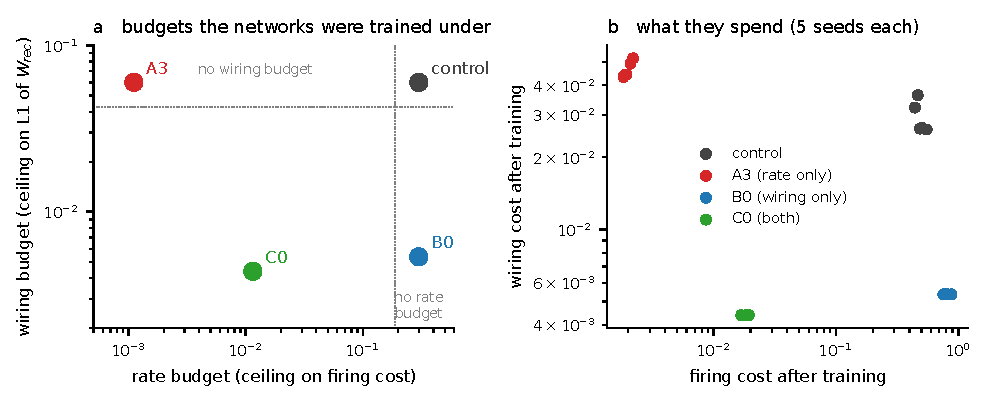
\includegraphics[width=\linewidth]{fig/fig1_points.pdf}
  \caption{\textbf{a}, the budgets of the four points (log axes; points drawn outside the dotted lines have no
  budget on that axis). \textbf{b}, firing and wiring cost of the trained networks, one dot per seed.}
  \label{fig:points}
\end{figure}

%--------------------------------------------------------------------------------------------------
\section{Finding task groups, separately for E and for I}

\paragraph{Task variance.} For every unit and every task we measure how much the unit's activity varies across
trials of that task (variance across trials at each time point, averaged over the trial), as in Yang et~al.\ (2019).
A unit with high task variance on a task carries information about that task. This gives a table of
20 tasks $\times$ 256 units. Units that barely vary on any task are dropped, and each remaining unit's 20 values are
divided by its own maximum, so every unit has a \emph{task profile} between 0 and 1 whose largest entry is 1.

\paragraph{Clustering.} Yang et~al.\ cluster all units together. Here E and I units are clustered
\emph{separately}: k-means on the task profiles of the E units, and independently on those of the I units. The
number of groups is chosen from the silhouette score, as Yang does. The result is a set of E groups and a set of I
groups, each with an average task profile. The top panels of Figs.~\ref{fig:control}--\ref{fig:C0} show these
groups: each column is a unit, each row a task, and white means the unit varies most on that task.

\paragraph{How broad are the neurons?} A simple number per population is the \emph{number of tasks per neuron}:
for how many of the 20 tasks a unit's profile is above half of its maximum. A unit that cares about one
task scores 1, a unit that is involved in everything scores 20.

%--------------------------------------------------------------------------------------------------
\section{Three ways E and I could be organised}

Once we have E groups (modules), there are three simple possibilities for the inhibitory neurons
(Fig.~\ref{fig:types}).

\begin{figure}[h]
  \centering
  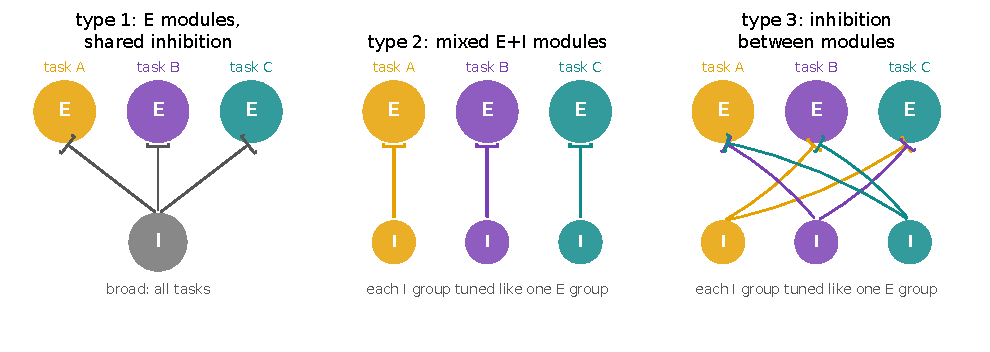
\includegraphics[width=0.95\linewidth]{fig/fig2_types.pdf}
  \caption{The three kinds of E/I organisation. Circles are groups of neurons, coloured by the task they are
  involved in; bars are inhibitory connections.}
  \label{fig:types}
\end{figure}

\textbf{Type 1: E modules with shared inhibition.} The task modules are purely excitatory. Inhibition is a
common pool that is active in all tasks and inhibits everyone, for instance to keep overall activity in check.
I neurons should then be broader than E neurons, and their connections should not care which task an E group
does.

\textbf{Type 2: mixed E+I modules.} Each module has its own excitatory and inhibitory neurons. An I group is tuned
to the same tasks as one E group and is wired mainly to that E group, in both directions: the E group drives its
I group, and the I group inhibits its own E group (local feedback inhibition).

\textbf{Type 3: inhibition between modules.} I groups are also tuned like E groups, but they inhibit the
\emph{other} modules. When one module is active it suppresses the competing ones (lateral inhibition).

Types 2 and 3 look the same when we only look at tuning: in both, every I group has an E group with the same task
profile. They differ only in the wiring, and that is what the next section measures.

%--------------------------------------------------------------------------------------------------
\section{Measuring whether the wiring follows the tasks}

For one network we compute two tables with one entry per pair of an I group and an E group
(Fig.~\ref{fig:method}, using C0 as the example):

\begin{enumerate}
  \item \textbf{Task similarity} (panel a): the correlation $r$ between the I group's and the E group's average
  task profile. $r$ near 1 means the two groups are involved in the same tasks.
  \item \textbf{Wiring strength} (panel b): the average absolute weight from every unit of the I group to every
  unit of the E group (synapses that were pruned count as 0). The raw number depends on group sizes and on how many
  synapses the network has overall, so we compare it with the same number after shuffling which unit belongs to
  which group (500 shuffles, group sizes kept) and report how many standard deviations it lies above the shuffles
  ($z$). $z = 0$ means the two groups are as connected as two random sets of neurons of the same size.
\end{enumerate}

Then we ask whether the two tables go together (panel c): the Spearman correlation $\rho$ between task
similarity and wiring strength over all (I group, E group) pairs of the network.

\begin{itemize}
  \item $\rho > 0$: I groups are wired most strongly to the E groups that do the same tasks \,$\to$ type 2.
  \item $\rho < 0$: I groups are wired most strongly to E groups that do \emph{different} tasks \,$\to$ type 3.
  \item $\rho \approx 0$: wiring ignores the tasks \,$\to$ type 1.
\end{itemize}

The same is done for the opposite direction, E $\to$ I. Type 2 predicts positive $\rho$ in both directions.

\begin{figure}[h]
  \centering
  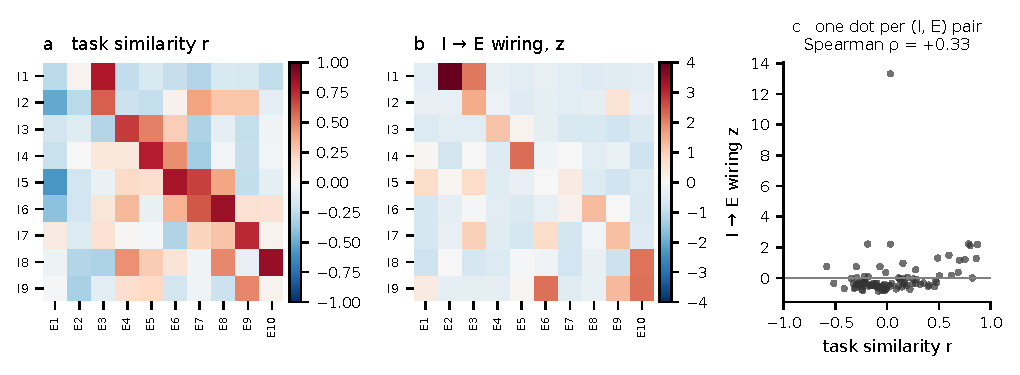
\includegraphics[width=\linewidth]{fig/fig3_method.pdf}
  \caption{The wiring measure for one network (C0, seed 2). \textbf{a}, task similarity of every I group (rows) with
  every E group (columns). \textbf{b}, I $\to$ E wiring strength as a $z$-score against shuffled groups.
  \textbf{c}, the two tables plotted against each other: one dot per (I group, E group) pair. Here the pairs that
  share tasks (right) tend to be more strongly connected, $\rho = +0.33$. One pair (I1 $\to$ E2) is far
  stronger than all others: a small I group projecting to the RT~Anti group.}
  \label{fig:method}
\end{figure}

%--------------------------------------------------------------------------------------------------
\section{Results}

For each point we show the seed with the best worst-task accuracy, and then check against the other four seeds
(Fig.~\ref{fig:summary}).

\subsection*{Control: inhibition between modules (type 3)}

The unconstrained network has few, broad E groups: about 5 tasks per neuron, and the groups are task
\emph{families} (all DM tasks, all delayed DM tasks, the matching tasks) rather than single tasks
(Fig.~\ref{fig:control}). The I neurons are tuned as narrowly as the E neurons, and every I group has an E group
with a similar profile.

The wiring shows the clearest effect of the four points: I $\to$ E $\rho$ is negative in all five seeds (between
$-0.3$ and $-0.7$). An I group inhibits the E groups of \emph{other} tasks more than chance, and its own E partner
less. The E $\to$ I direction is unstructured ($\rho$ around 0). This is lateral inhibition between modules.

Note that the control keeps two thirds of all synapses, so here the measure is about how \emph{strong} the
synapses are, not about whether they exist.

\begin{figure}[p]
  \centering
  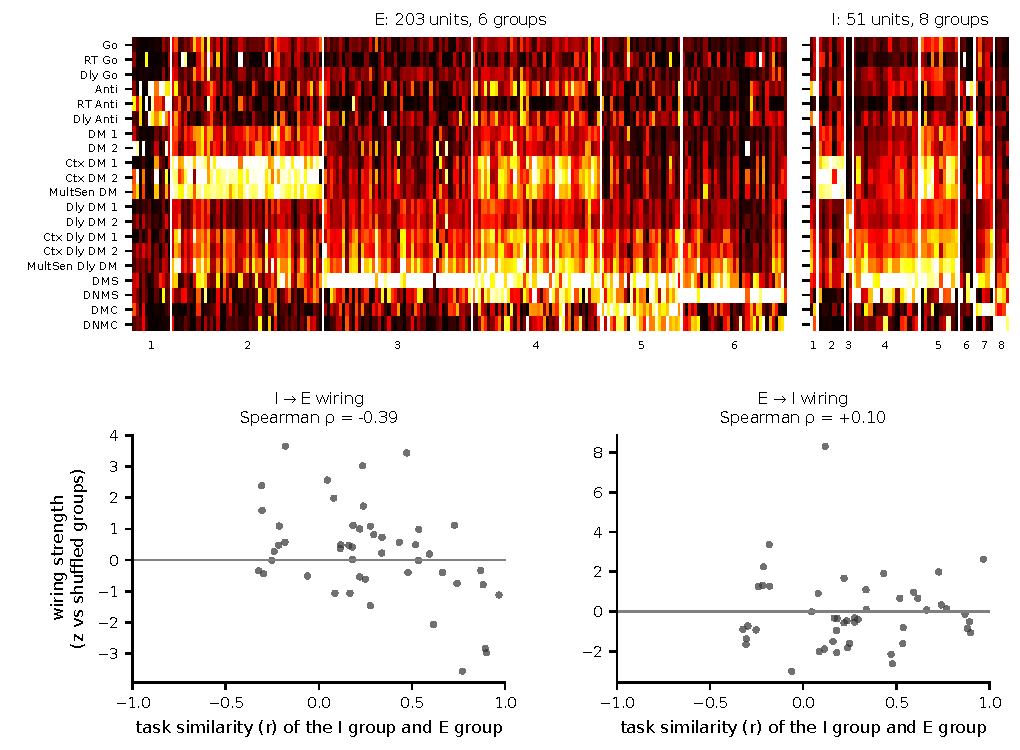
\includegraphics[width=0.92\linewidth]{fig/fig_net_control.pdf}
  \caption{Control, seed 1. Top: normalised task variance of the active E units (left) and I units (right), units
  sorted by group. Bottom: wiring strength against task similarity for every (I group, E group) pair, for
  I $\to$ E and E $\to$ I.}
  \label{fig:control}
\end{figure}

\subsection*{A3, rate only: sharp E modules, wiring ignores tasks}

Limiting firing gives the most specialised E neurons of all four points: about 3 tasks per neuron, and many small
E groups, several of them dedicated to a single task (RT~Go, RT~Anti, DMS, DNMS, DMC; Fig.~\ref{fig:A3}). The I
neurons do not follow this: in every seed they are broader than the E neurons (about 4 tasks per neuron) and fall
into fewer groups. Their profiles still resemble an E group, but at the level of task families (for example all
delayed tasks) rather than single tasks.

The wiring does not follow the tasks at all: $\rho$ is within $\pm 0.06$ of zero for I $\to$ E in every seed, and
around zero for E $\to$ I. Like the control, A3 keeps most synapses, so this is again about weight strength.

A3 is therefore closest to type~1: the excitatory network is modular, while inhibition is broader and not wired
to particular modules.

\begin{figure}[p]
  \centering
  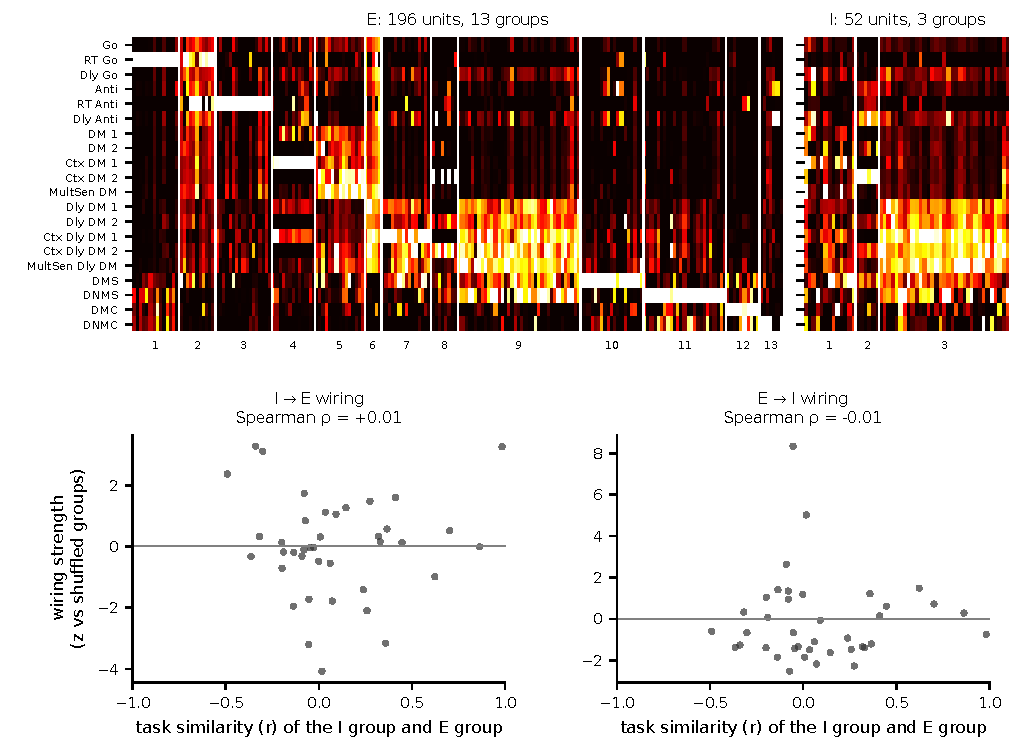
\includegraphics[width=0.92\linewidth]{fig/fig_net_A3.pdf}
  \caption{A3 (rate only), seed 3. Same layout as Fig.~\ref{fig:control}.}
  \label{fig:A3}
\end{figure}

\subsection*{B0, wiring only: weak, seed-dependent E+I pairing}

With only a wiring budget the E neurons are the broadest of the four points (about 5 tasks per neuron), and the
E groups are few and large (four in the seed shown, Fig.~\ref{fig:B0}). The task structure is the weakest here.

The wiring tends to be positive in both directions, $\rho \approx +0.2$ on average, but the seeds disagree:
only two of the five seeds are clearly positive in both directions, the others are close to zero in at least one. This is a weak hint of type 2, not a clear
result. Unlike the control and A3, only 6\,\% of synapses remain, so here the measure also reflects which
synapses exist.

\begin{figure}[p]
  \centering
  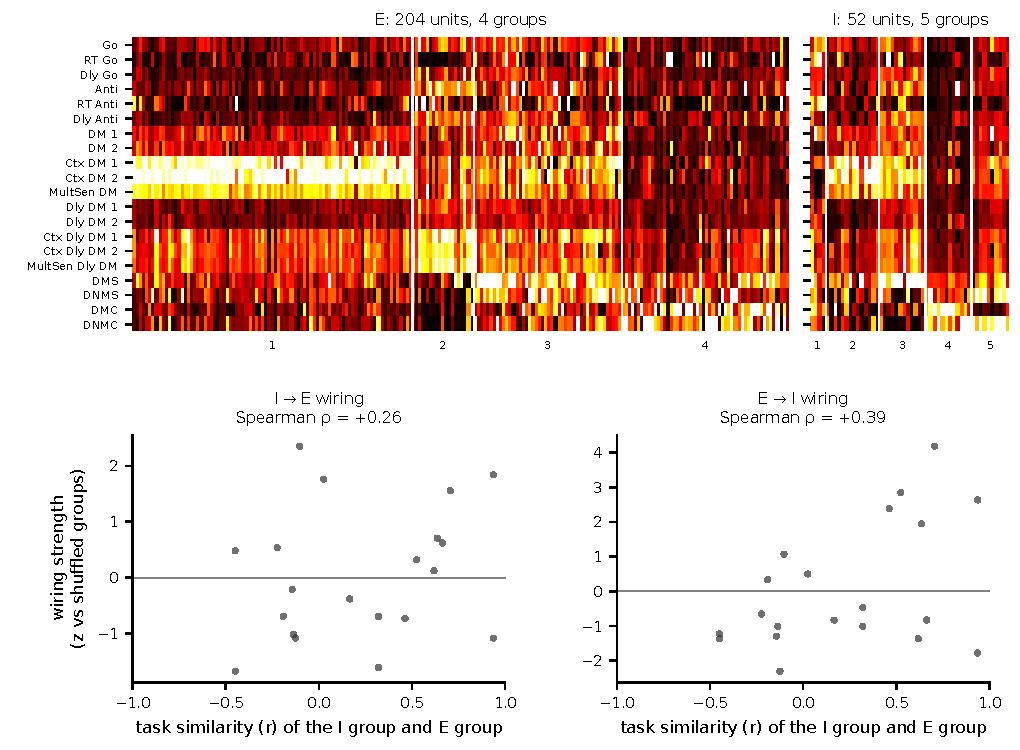
\includegraphics[width=0.92\linewidth]{fig/fig_net_B0.pdf}
  \caption{B0 (wiring only), seed 0. Same layout as Fig.~\ref{fig:control}.}
  \label{fig:B0}
\end{figure}

\subsection*{C0, both budgets: mixed E+I modules (type 2)}

With both budgets the E neurons are sharply tuned (about 3.5 tasks per neuron) and form many groups, close to
A3. Unlike A3, the I neurons are only slightly broader than the E neurons (about 4 tasks per neuron)
and form more groups (Fig.~\ref{fig:C0}).

Here the wiring follows the tasks. E $\to$ I $\rho$ is clearly positive in all five seeds (between $+0.3$ and
$+0.6$): an E group connects mostly to the I groups that are involved in the same tasks. The I $\to$ E direction
is positive in all five seeds as well, but weaker ($+0.1$ to $+0.3$). With less than 1\,\% of synapses left,
this is a statement about which connections the network kept. C0 is the only point that matches type 2 in both
tuning and wiring.

\begin{figure}[p]
  \centering
  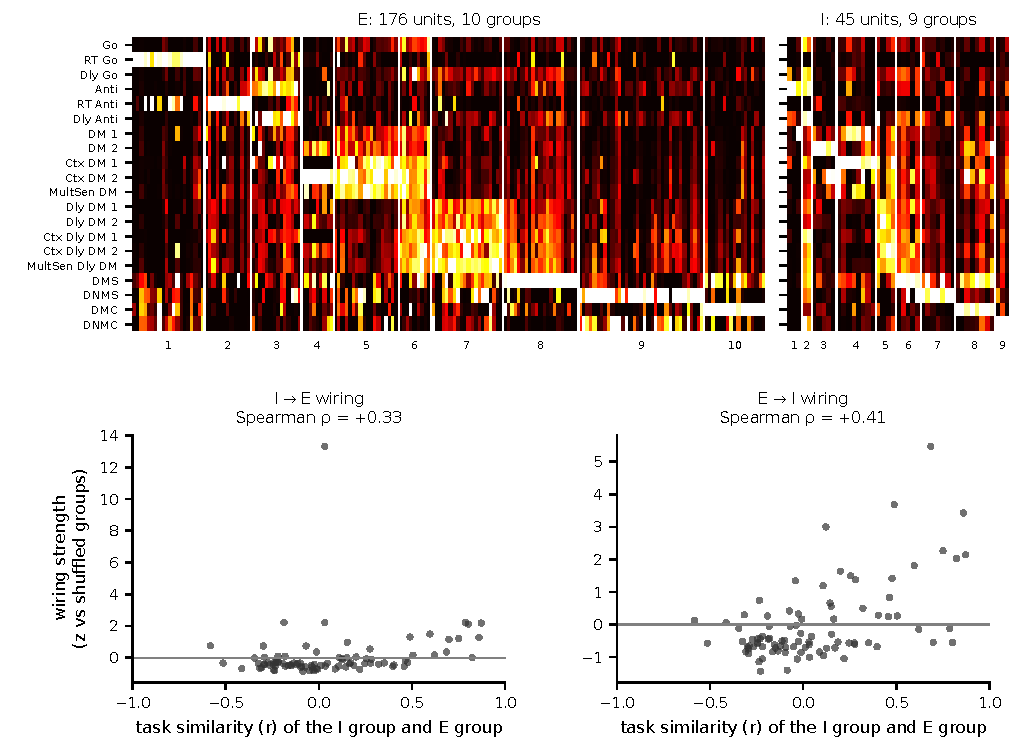
\includegraphics[width=0.92\linewidth]{fig/fig_net_C0.pdf}
  \caption{C0 (both budgets), seed 2. Same layout as Fig.~\ref{fig:control}.}
  \label{fig:C0}
\end{figure}

%--------------------------------------------------------------------------------------------------
\clearpage
\section{Summary}

\begin{figure}[h!]
  \centering
  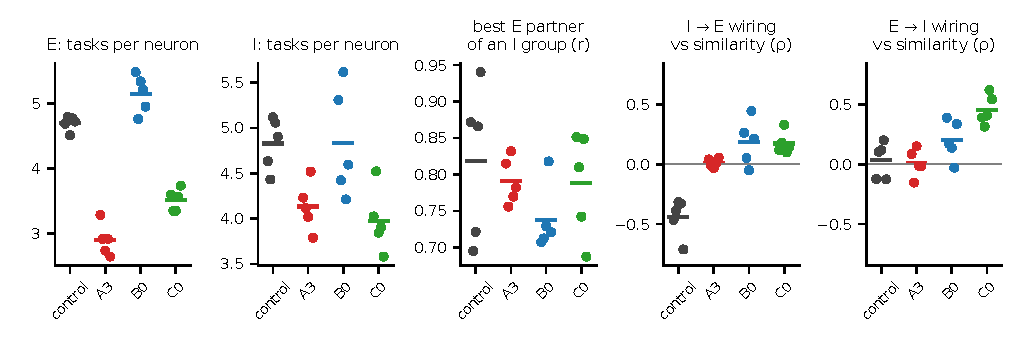
\includegraphics[width=\linewidth]{fig/fig4_summary.pdf}
  \caption{The five numbers of this note for all 20 networks. Dots are seeds, bars are means over the 5 seeds.}
  \label{fig:summary}
\end{figure}

\begin{table}[h]
  \centering
  \small
  \begin{tabular}{lcccc}
    \toprule
    & control & A3 (rate) & B0 (wiring) & C0 (both) \\
    \midrule
    E tasks per neuron & 4.7 & 2.9 & 5.2 & 3.5 \\
    I tasks per neuron & 4.8 & 4.1 & 4.8 & 4.0 \\
    I $\to$ E wiring vs task similarity ($\rho$) & $-0.44$ & $0.01$ & $0.19$ & $0.18$ \\
    E $\to$ I wiring vs task similarity ($\rho$) & $0.04$ & $0.01$ & $0.20$ & $0.46$ \\
    synapses kept & 70\,\% & 61\,\% & 6\,\% & 0.7\,\% \\
    \midrule
    closest type & 3 & 1 & weak 2 & 2 \\
    \bottomrule
  \end{tabular}
  \caption{Means over 5 seeds.}
\end{table}

Read together:

\begin{itemize}
  \item Without budgets, the network forms broad modules that \textbf{inhibit each other} (type 3).
  \item A \textbf{rate budget} sharpens the excitatory modules, but inhibition stays broader and is not wired
  to them (closest to type 1).
  \item A \textbf{wiring budget} alone makes neurons broad and gives at most a weak E+I pairing.
  \item \textbf{Both budgets together} give sharp excitatory modules \textbf{with their own inhibitory
  neurons}, wired to them mainly in the E $\to$ I direction (type 2).
\end{itemize}

Every I group in every network has an E group with a similar task profile (best match $r \approx 0.7$--$0.9$
everywhere), so the four points differ in the breadth of I tuning and above all in the wiring, not in whether
the I neurons are tuned at all.

\paragraph{Caveats.}
Five seeds per point. Each network's $\rho$ is computed from its own groups, between about 12 and 170 (I, E)
pairs, and the number of groups changes from seed to seed. We only make claims where the seeds barely overlap:
the negative I $\to$ E $\rho$ of the control, the positive E $\to$ I $\rho$ of C0, the zero wiring $\rho$ and
broader I neurons of A3. In the control and A3 almost every synapse exists, so their wiring numbers describe
weight strength only. Lesion experiments, which test whether the I part of a module is actually needed, are
in the notebook and not discussed here.

\end{document}
